\chapter{Results and discussion}

This chapter reports the detail of the analysis procedures which include
% The content of this chapter would be reported as the analysis 
% procedure from step one to the end. The first part is
the data correction process, count maps from the raw count,  
exposure map from the parallel computation, the spectrum calculation,
and inversive fitting of the spectral models from heuristic optimization.

\section{Limb angle correction}
% Theoretically, the peak profile of the $\theta_\text{NADIR}$ would be
% the same when time passes by.
From the observations, the
peak of the Earth's limb $\gamma$-ray $\theta_{\rm NADIR}$ profile changes over time
% nadir angle change through time evolving
since the spacecraft altitude is gradually getting lower each
year, effectively increasing the peak position of $\theta_{\rm NADIR}$
from the LAT's point of view.
% year which will affect the LAT point of view when it sees 
% the Earth.

\begin{figure}[h!]
    \centering
    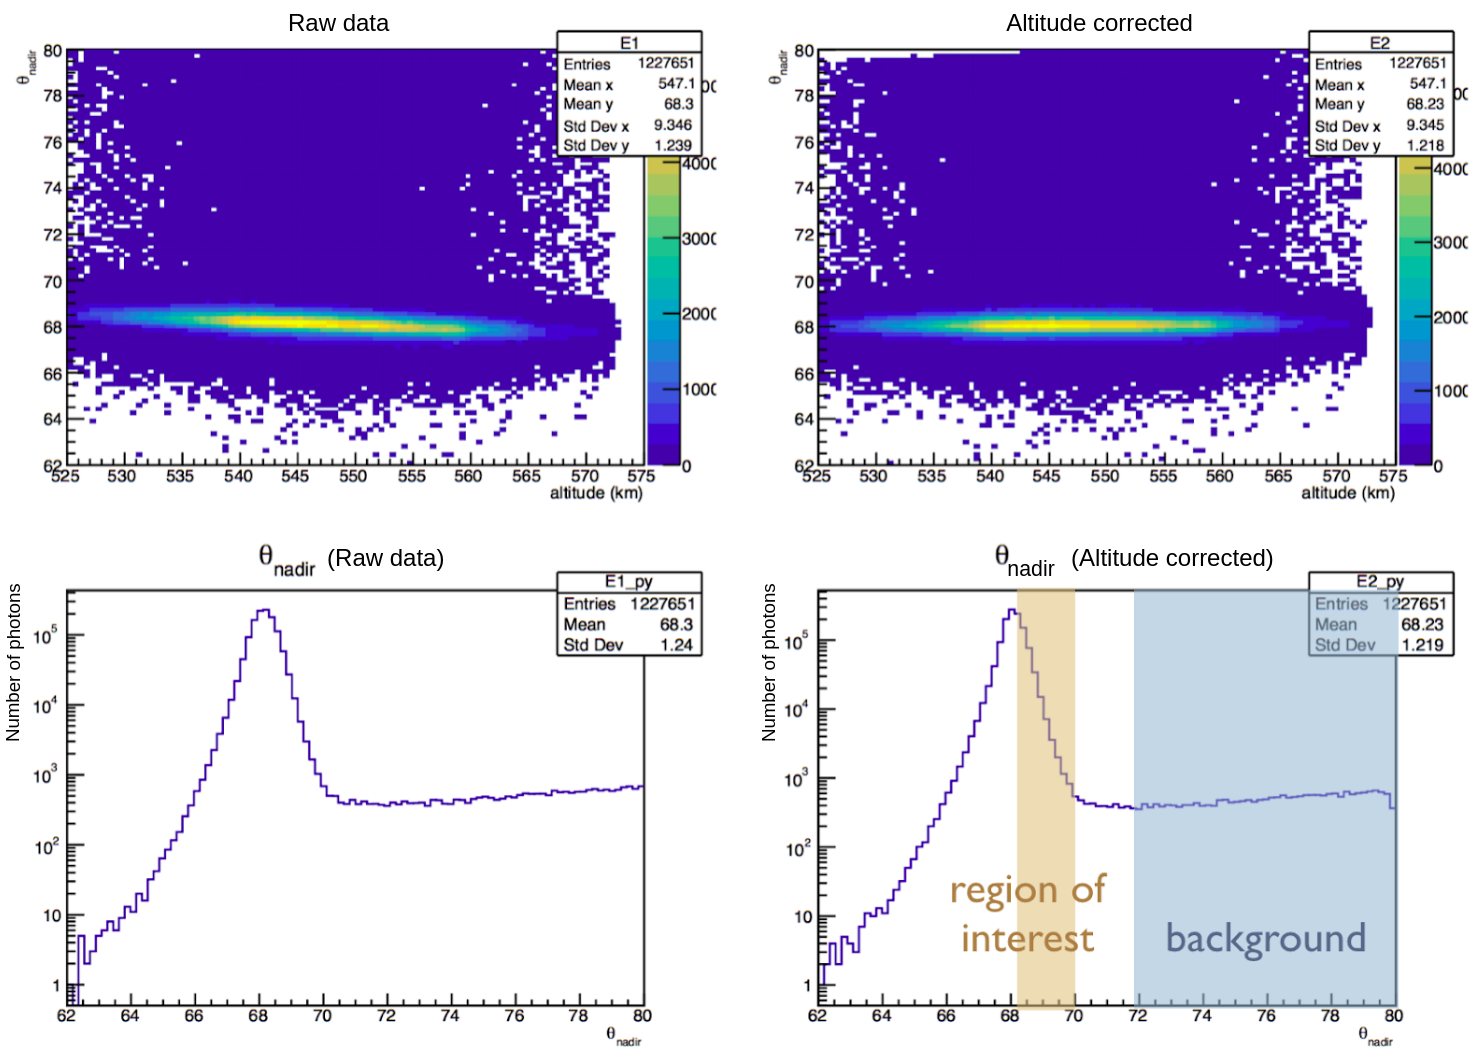
\includegraphics[width=0.8\textwidth]{content/result_and_discussion/figures/LATShifted_v3.png}
    \caption{
        Distribution of number of photons above 20 MeV with nadir angle
        ($\theta_{\rm NADIR}$) before (left) and after (right)
        altitude correction.
        Top panels show 2D histograms of number of photons in
        each $\theta_{\rm NADIR}$ and altitude (in km) bin.
        Bottom panels show the projection of the 2D histograms
        in the top panels onto the $\theta_{\rm NADIR}$ axis
        in which photons from all altitudes are accumulated
        into each $\theta_{\rm NADIR}$ bin.
        % Distribution of nadir angle before and after altitude correction.
        % (top) Heatmaps represents the photon density in axis
        % of $\theta_\text{NADIR}$ versus altitude in kilometers.
        % The left one came from raw data and the right one was
        % converted by altitude shifting calculation.
        % (bottom) The projected histograms from the above heatmaps
        % in the axis of $\theta_\text{NADIR}$ where all photon
        % from various altitudes was accumulated into the bin value.
    }
    \label{fig:lat_nadir_shifted}
\end{figure}


The top-left of Figure \ref{fig:lat_nadir_shifted} demonstrates how 
spacecraft orbiting altitude
affects the $\theta_{\rm NADIR}$ profile by showing a 2D histogram
of photon count in each altitude and $\theta_{\rm NADIR}$ bin.
% correlates to the $\theta_\text{NADIR}$
% by a 2D heatmap plot of photon intensity.
The bottom-left plot is the projection of the
previous raw count 2-D histogram
onto the $\theta_{\rm NADIR}$ axis which shows
% which has
a peak around 68\textdegree. Both bottom and top right histograms
are constructed in a similar idea but with the spacecraft altitude
correction on the $\theta_{\rm NADIR}$ which reduce the effect
of the LAT orbital decay over time. The region of interest used
to calculate the Earth's limb $\gamma$-ray spectrum is
highlighted in orange, and the region highlighted in blue
gives an estimate of the background photons which is subtracted
from the limb flux. Note that the Earth's limb emission is
approximately one order of magnitude brighter than the background
emission.
% were constructed from the same logic but there is one different 
% variable. The shifted nadir angle has been calculated to reduce the 
% effect from the spacecraft and the region of interest has been highlighted 
% as orange for calculating as the limb spectrum and the blue zone is 
% a diffusive background to be used in the background subtraction.

% The brightness of Earth's limb is much brighter than the 
% diffusive background on the map. The region of interest and 
% the background intensity has a huge difference in approximately
% an order of magnitude.


\section{Earth's limb $\gamma$-ray spectrum measurement}

According to Equation \ref{eq:def_flux}, 
the first step is the construction of
count maps in the local zenith coordinates.
Visualization of a raw count map above 10 GeV from 1 week of
data is demonstrated in Figure \ref{fig:sample_photon_dist}.
% the count map of the Earth's 
% centered coordinates. To illustrate how the outcome looks like,
% we selected photon data from a single week due to the raw data
% of photon from \textit{Fermi} was published once a week as one file.
% A week of the accumulated photons is plotted in
% Figure \ref{fig:sample_photon_dist} to visualize 
% the raw count of the sample data on the count map.

\begin{figure}[h!]
    \centering
        \subfloat[
            2D histogram of >10 GeV photons binned in nadir angle
            ($\theta_{\rm NADIR}$) along the radial direction
            and azimuthal angle ($\phi_{\rm NADIR}$) along
            the azimuthal direction.            
            % Heatmap of photon density in nadir angle where the 
            % radius direction is the azimuthal nadir
            % angle ($\theta_\text{NADIR}$).
        ]{
            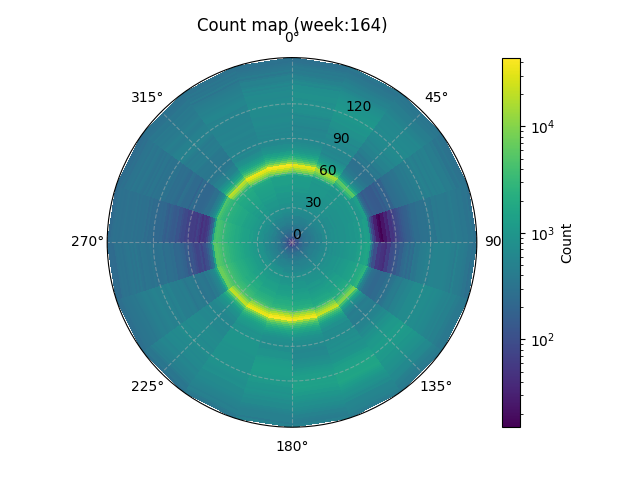
\includegraphics[width=0.47\textwidth]{content/result_and_discussion/figures/cntmap_polar.png}
        }
        \hfill
         \subfloat[
            Distribution of photon counts with
            $\phi_{\rm NADIR}$ for
            $0^\circ<\theta_{\rm NADIR}<150^\circ$.
            % (ควรจะมีระบุขอบเขตของ theta_NADIR ด้วย)
            % A projected histogram from the heatmap.
            % The x-axis is $\phi_\text{NADIR}$ from 0\textdegree
            % to 360\textdegree.
        ]{
            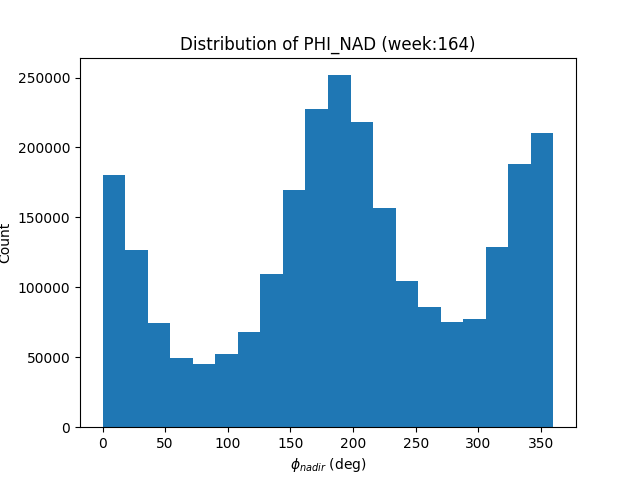
\includegraphics[width=0.47\textwidth]{content/result_and_discussion/figures/phi_nad_dist.png}
        }
        \caption{
            An example distribution of
            $\gamma$ rays above 10 GeV from 1 week of LAT data
            % $\gamma$-ray from a single week.
        }
       \label{fig:sample_photon_dist}
\end{figure}

The limb's region could be easily observed in the bright ring
at $\theta_{\rm NADIR}\approx68^\circ$.
% above a dashed line at $\theta_\text{NADIR}=60^\circ$.
% of 60\textdegree  $\theta_\text{NADIR}$.
Figure \ref{fig:sample_photon_dist} shows more
brightness from the north and south limb
due to the LAT's survey mode configuration which results in
higher exposure in the north and south regions.
Projection of the 2D histogram in
Figure \ref{fig:sample_photon_dist}a onto a 1D histograms
of the azimuthal angle ($\phi_{\rm NADIR}$) is shown in Figure
\ref{fig:sample_photon_dist}b which roughly
illustrates the East-West effect
(more photons from the West) although the exposure has not
been taken into account yet. The asymmetric distribution
could caused from the asymmetric exposure which will be 
investigated later in this section.
% Figure \ref{fig:sample_photon_dist} also shows the brightness of 
% the southern and northern hemispheres.
% Further investigating of the 
% East-West effects could be illustrated by projecting the 2-D histogram 
% into a 1-D histogram of the nadir angle as in Figure \ref{fig:sample_photon_dist}b.
To illustrate the East-West effect in $\gamma$-ray,
projecting the photon intensity into $\phi_\text{NADIR}$ axis is 
visualized in Figure \ref{fig:flx_phi}.

% Applying criteria from the data selection such as event class,
% LAT's incident angle would affect the result from
% the histogram filling.


\begin{figure}[h!]
    \centering
    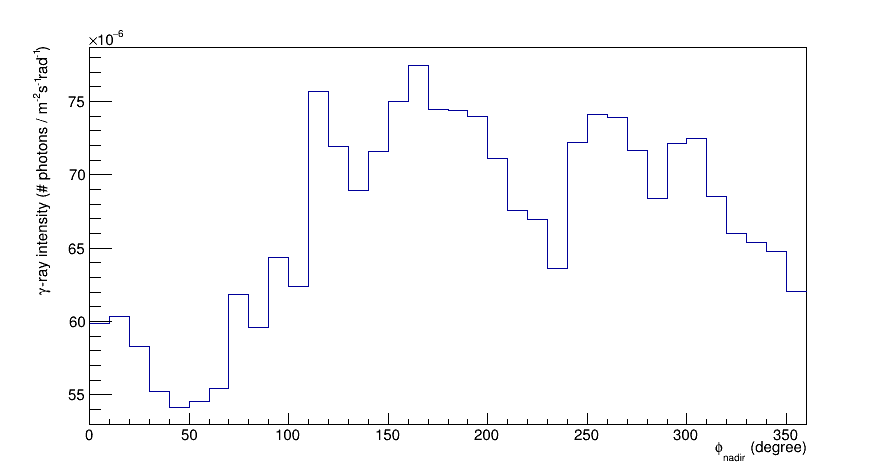
\includegraphics[width=0.9\textwidth]{content/result_and_discussion/figures/zoom_rs/flx_phi_nadir_hist.png}
    \caption{Earth's $\gamma$-ray intensity in $\phi_\text{NADIR}$ axis}
    \label{fig:flx_phi}
\end{figure}


% \begin{figure}[h!]
%     \centering
%     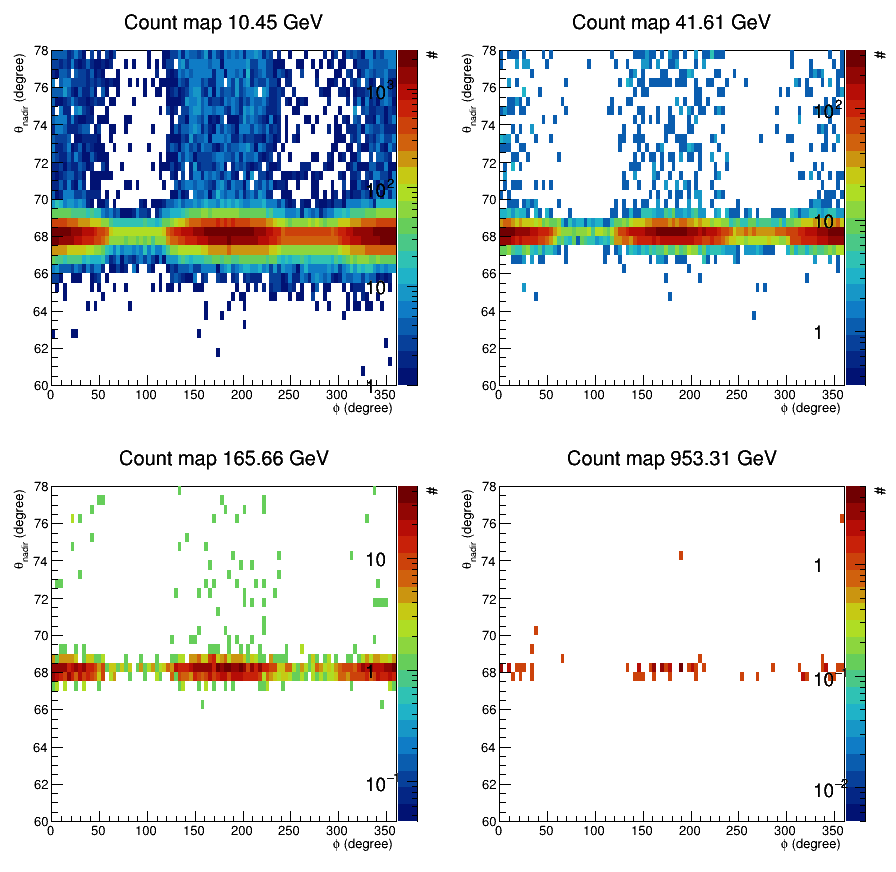
\includegraphics[width=0.8\textwidth]{content/result_and_discussion/figures/zoom_rs/cartesian_cntmaps.png}
%     \caption{
%         Cartesian plot of the $\gamma$-ray count histograms.
%         The title each sub-figure represents
%         mean of the energy bins.
%     }
%     \label{fig:cntmap_cartesian}
% \end{figure}

% Since the final spectrum will contain 50 energy bins
% with their specific energy range and mean energy
% for each energy bin.
% In practice, each heatmap will be constructed
% for their belonging bin of the histogram in the energy domain
% as in Figure \ref{fig:cntmap_cartesian}.


% However, inspecting at polar coordinate plotting
% from the cartesian point of view might not be the best option for 
% illustration since it not looks like the real orientations.
Figure \ref{fig:cntmap_polar} shows the count maps in 4 energy bands
(as examples from 50 bands total) in the local zenith coordinate
system where the Earth is placed at the center of each map.
The limb emission can be seen clearly as shiny thin rings
which become dimmer at higher energy.
% Figure \ref{fig:cntmap_polar} is another
% angle of viewing the same data but in more natural orientations.
% Both visualizations show that the Earth's limb region in $\gamma$-ray 
% is the shinest band for all interesting energy.
% It is also obvious to say that the higher energy scale,
% the less photon appears after applying criteria.


\begin{figure}[h!]
    \centering
    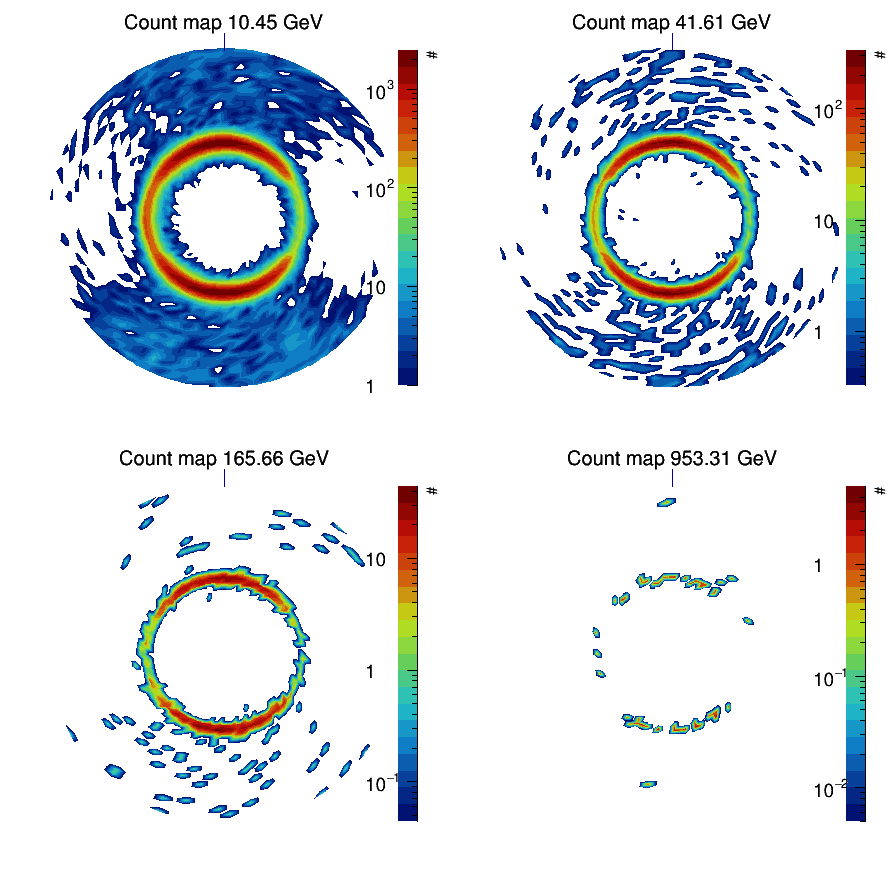
\includegraphics[width=0.8\textwidth]{content/result_and_discussion/figures/zoom_rs/polar_cntmaps.png}
    \caption{
        Count maps in the local zenith coordinates.
        The bright emission ring
        is located at the limb ($\theta_{\rm NADIR}\approx68^\circ$).
        The radial axis is in range $60^\circ<\theta_{\rm NADIR}<80^\circ$
        and the clockwise direction is starting from $\phi_{\rm NADIR}=0^\circ$ 
        to $\phi_{\rm NADIR}=360^\circ$ .
    }
    \label{fig:cntmap_polar}
\end{figure}


The next step is the exposure calculation.
The exposure map is computed 
by accumulating exposure time from the LAT's FoV
in each time step as well as takes
in to account the detector efficiency as a function
of incident angle and energy.
% the effectiveness of the detector due to incident angle
% affects the performance of the detector.
Examples of exposure maps, for which the unit is area $\times$ time,
are shown in Figure \ref{fig:expmap_cartesian}.
% A unit from the calculation will be an 
% area multiple by the time. Raw cartesian plots are visualized in
% Figure \ref{fig:expmap_cartesian} with an attached axis.

% \begin{figure}[h!]
%     \centering
%     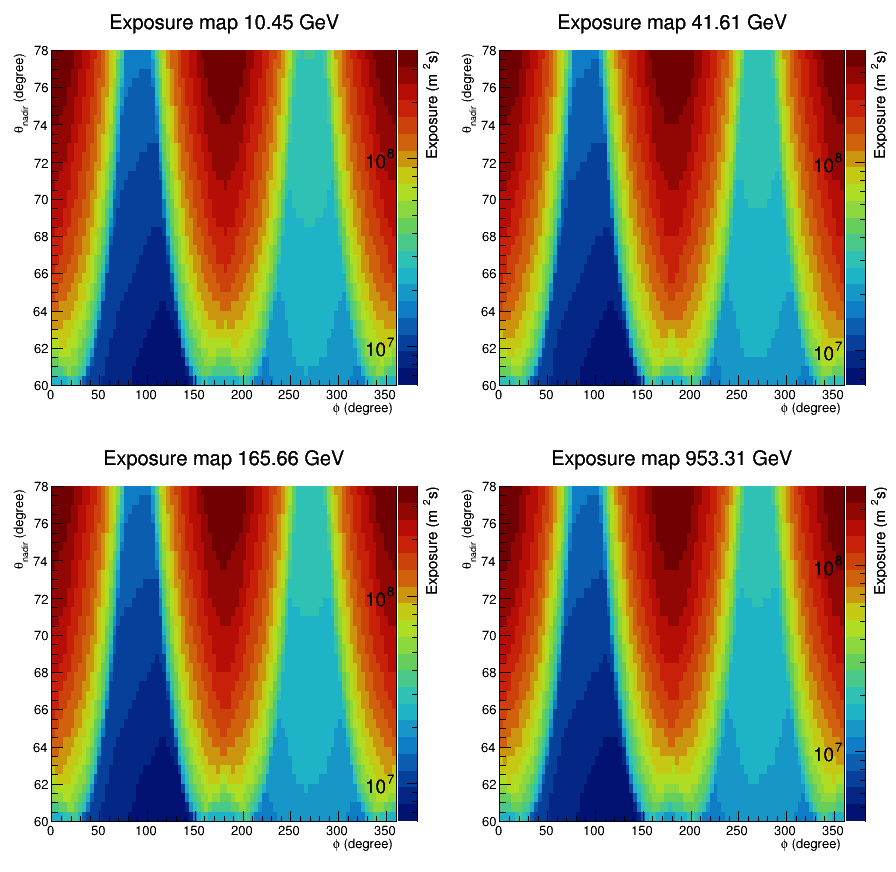
\includegraphics[width=0.8\textwidth]{content/result_and_discussion/figures/zoom_rs/cartesian_expmaps.png}
%     \caption{Cartesian plot of the exposure histograms.}
%     \label{fig:expmap_cartesian}
% \end{figure}


Examples of exposure maps in local-zenith coordinates are
shown in Figure \ref{fig:expmap_polar}, indicating that the sky exposure
(region near the edge of the each plot) is an order of
magnitude higher than that for the Earth because the LAT
is configured to survey the sky and avoid pointing directly at Earth.
Regarding the exposure of the Earth's limb region
($\theta_{\rm NADIR}\approx68^\circ$), the north and south exposure
is higher than that for the east and west because of the LAT's survey
configuration which switches between pointing north and south of
its orbital plane every orbit. The exposure of the western limb
is slightly higher than that of the eastern limb.
% The exposure intensity in the sky is much
% higher than the Earth in an order of magnitude
% because \textit{Fermi} was designed
% for seeking flare events in space rather than the Earth.
% Regarding a given nadir angle between
% 60\textdegree to 70 \textdegree,
% the spacecraft seems to look at the northern and southern hemispheres 
% more than the eastern and the western side. The color of the 
% at 270\textdegree (West) is more intense than 90\textdegree (East)
% means that the spacecraft tends to peek in the Westside more
% than Eastside. The reason might come from the
% trajectory of the charged particles was bent
% and produce a $\gamma$-ray which potentially could 
% convince \textit{Fermi} to look at them rather
% than the other side because it 
% has a more for triggering the GBM.
% The 2-D histograms in polar coordinates have also been
% plotted in Figure \ref{fig:expmap_polar}.

\begin{figure}[h!]
    \centering
    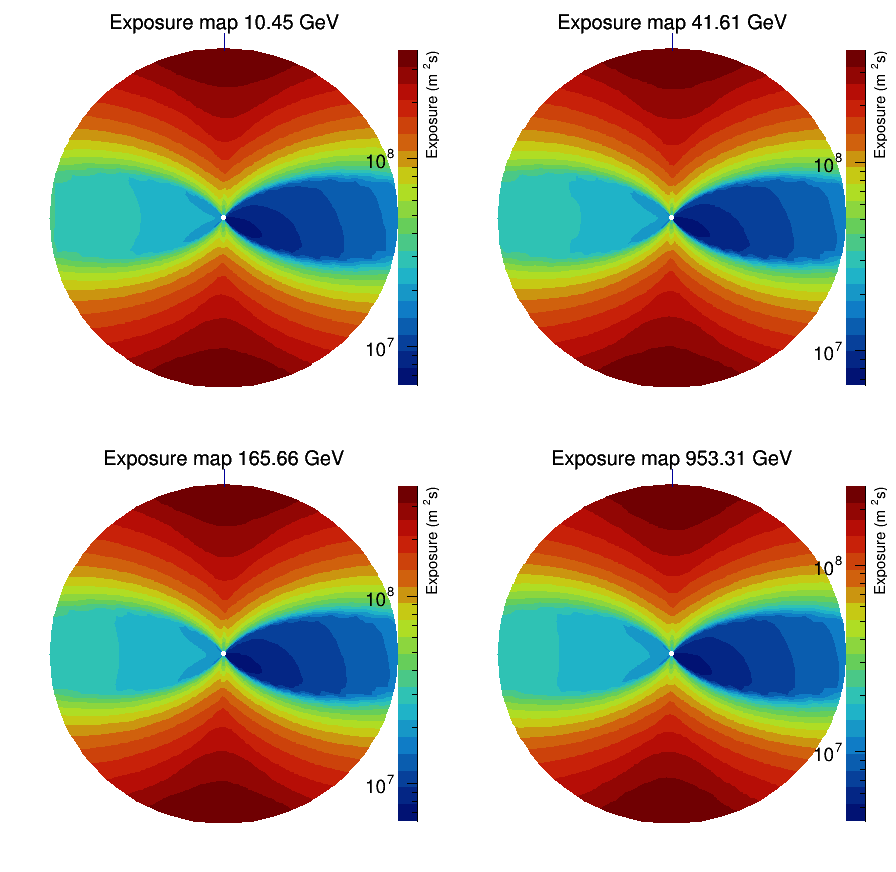
\includegraphics[width=0.8\textwidth]{content/result_and_discussion/figures/zoom_rs/polar_expmaps.png}
    \caption{
        Exposure maps in local-zenith coordinates in 4 energy bands.
        The Earth's limb is indicated by the dotted circle in which
        the north, east, south, and west part of the limb are labeled. 
        % Polar plot of the exposure histograms.
    }
    \label{fig:expmap_polar}
\end{figure}

\begin{figure}[h!]
    \centering
    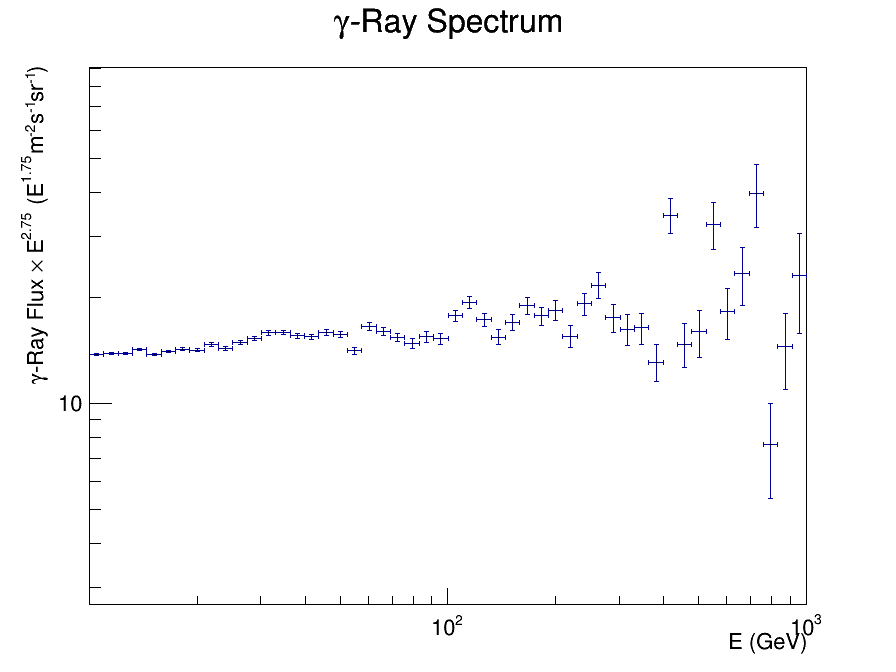
\includegraphics[width=0.7\textwidth]{content/result_and_discussion/figures/flx_hist.png}
    \caption{
        Measured Earth's limb $\gamma$-ray spectrum
        from $68.4^\circ<\theta_{\rm NADIR}<70.0^\circ$ by this work.
        % Measured $\gamma$-ray spectrum.
    }
    \label{fig:flxhist}
\end{figure}


To obtain flux maps, we divide the count by the exposure maps bin by bin.
We integrate the flux map in the limb region
($68.4^\circ<\theta_{\rm NADIR}<70.0^\circ$) and
divide by the energy bin width and the solid angle size of the region
to obtain a spectral value for that energy bin.
After repeating the calculation for 50 energy bins
and subtracting the background flux from the sky
(see Figure \ref{fig:lat_nadir_shifted}),
we have the final Earth's $\gamma$-ray spectrum as illustrated
in Figure \ref{fig:flxhist}.
% The last step starts with initiating the new heatmaps that were 
% defined by the element-wise division from the
% count maps and the exposure maps (Equation~\ref{eq:def_flux}).
% After that, integrating the limb region in the polar coordinates
% to get a single scalar value. The scalar is then divided by the 
% gap of the energy bin and the solid angle.
% Repeating the above process for 50 energy bins in the $\gamma$-ray 
% spectrum and subtracts by the background would yield the final 
% photon spectrum as in Figure \ref{fig:flxhist}.


% \begin{figure}[h!]
%     \centering
%     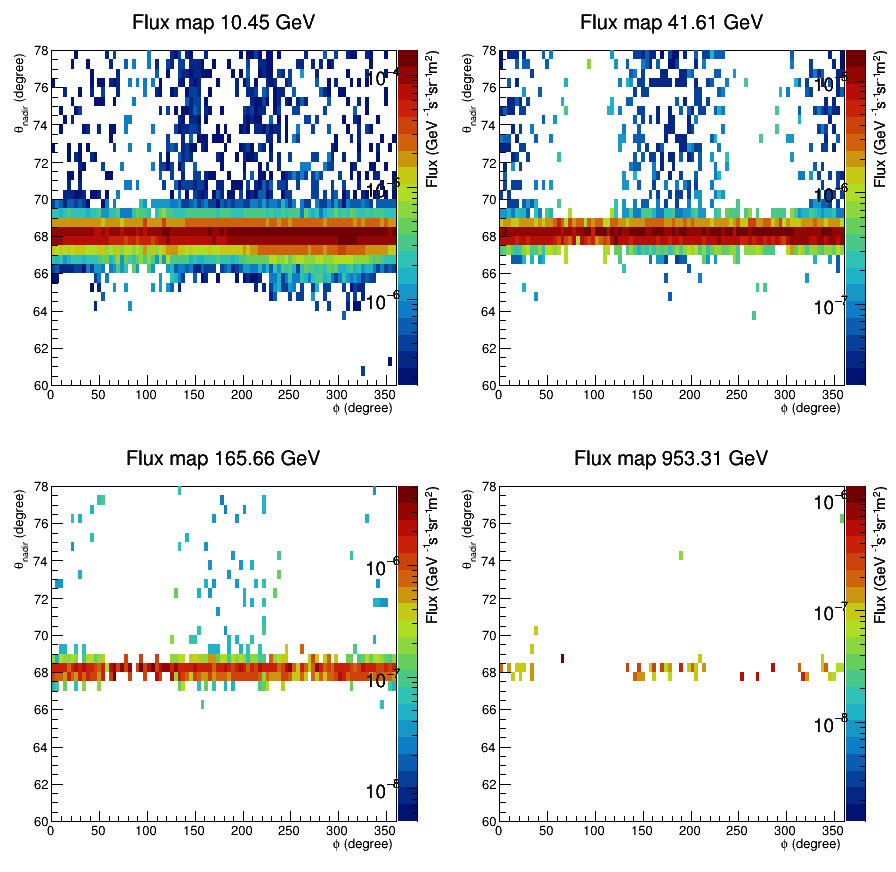
\includegraphics[width=0.8\textwidth]{content/result_and_discussion/figures/zoom_rs/cartesian_flxmaps.png}
%     \caption{Cartesian plot of the $\gamma$-ray flux histograms.}
%     \label{fig:flxmap_cartesian}
% \end{figure}


\begin{figure}[h!]
    \centering
    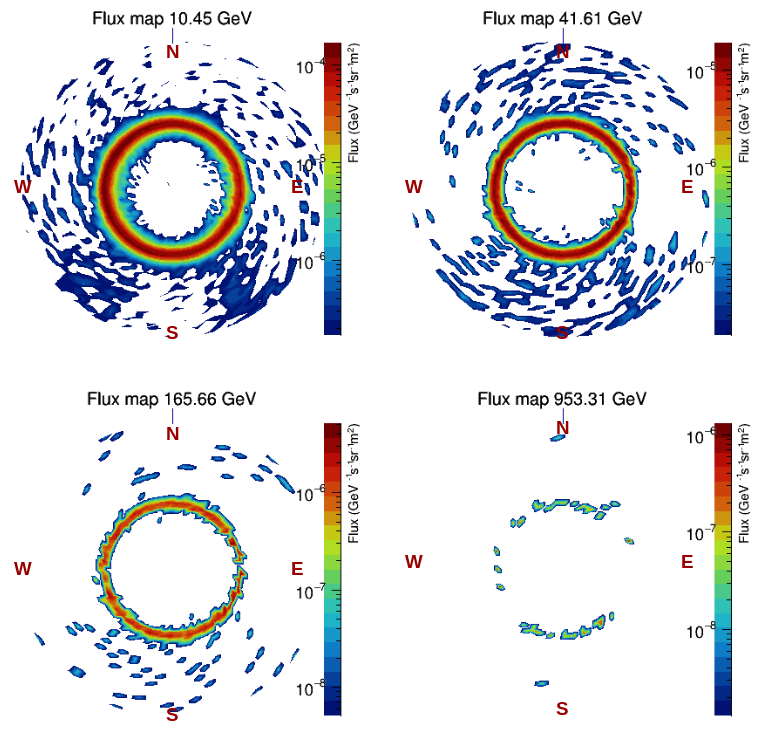
\includegraphics[width=0.8\textwidth]{content/result_and_discussion/figures/zoom_rs/polar_flxmaps_with_label.png}
    \caption{
        Flux maps of of the Earth's $\gamma$-ray emission in
        local zenith coordinates where the Earth is at the center
        of each panel and the ring is the $\gamma$-ray emission
        from the limb.
        % Polar plot of the $\gamma$-ray flux histograms.
    }
    \label{fig:flxmap_polar}
\end{figure}

Examples of $\gamma$-ray flux maps in local zenith coordinates
are visualized in Figure \ref{fig:flxmap_polar}, clearly showing
the bright ring-like emission from the Earth's limb.
The East-West effect can be observed from the thicker emission region
and brighter flux from the west limb.
% In addition, exploring the $\gamma$-ray
% intensity from the visualization
% of the Earth's centered coordinates would be informative aspects
% to observe the variation of the photon
% intensity along the nadir angle as well as the 
% East-West effect. The cartesian plotted as in Figure
% \ref{fig:flxmap_cartesian} and the polar form as in the Figure 
% \ref{fig:flxmap_polar}.Comparing the intensity along the peak of 
% theta nadir in the cartesian plot from the East ($\phi$=90\textdegree)
% and West ($\phi$=270\textdegree) would reflect that the band of 
% the intensity in the west is slightly
% thicker than in the East and the 
% color of the peak center is more a little darker than the other 
% side.
It means that not only is the intesity brighter
but also the ring thickness
of the limb region is larger from the west compared to those from the east.


As it can be seen that the expsoure maps where the north and south is 
much higher than the east and west which caused from the orbit 
orientation of the spacecraft. It is suspected 
that the measured $\gamma$-ray spectrum might not a robust results 
from some vanishing area in the calculation. The above clue leads
this work to perform another parallel study where the $\gamma$-ray 
from the Earth's limb takes only north and south direction into account.
The study in Appendix \ref{appendix:ns_analysis} was done by applying 
filter $\phi_\text{NADIR}$ from 330\textdegree to 30 \textdegree
as well as between 150\textdegree and 210\textdegree.


\section{Best fit results}

The optimized parameters for Single Power Law (SPL)
and Broken Power Law (BPL) models are summarized in 
Table \ref{tb:bestfit}. Best fit $\gamma$-ray 
spectra from both models are
% from both models is 
visualized in Figure \ref{fig:fitted_gamma_specgtrum} along
with the Earth's $\gamma$-ray spectrum from the measurement.
Our best fit BPL result is consistent with direct measurements
by AMS-02 \citep{AMS02pr2015} and PAMELA \citep{adriani2011pamela}
which identify
the CR proton spectral breaking at ~300 GeV as qualitatively
illustrated in Figure \ref{fig:fitted_cr_proton}.
% The result shows the consistency
% between the direct measurement from AMS-02 and
% the previous work.
Our results are also consistent with the indirect measurement
by the LAT \cite{FermiEarth14} which reported the best-fit BPL spectral
indices of $\Gamma_1\approx2.81$, $\Gamma_2\approx2.61$,
and the break energy at 302 GeV.
% Both studies identify the breaking point 
% of the spectral index in proton spectrum at $\sim$ 300 GeV,
% as well as the previous work, reported $\Gamma_1 \sim 2.81$
% and $\Gamma_2 \sim 2.68$ for the BPL model.

\begin{table}[h!]
    \centering
    \begin{tabular}{l | c | c | c}
      Best fits & $\Gamma_1$ & $\Gamma_2$ & $E_{\text{Break}}$ (GeV) \\
      \hline \hline
      SPL & 2.70 $\pm$ 0.08 (0.06) & - & -  \\
      BPL & 2.86 $\pm$ 0.14 (0.08) & 2.63 $\pm$ 0.13 (0.10) & 333 $\pm$ 10 (9)
    \end{tabular}
    \caption{
        % Optimization results.
        Optimized parameters for the SPL and BPL models for
        CR protons from this work where $\Gamma_1$ and $\Gamma_2$
        are spectral indices below and above
        the break energy ($E_{\rm Break}$), respectively.        
        Reportoed deviation is reported in total error
        and the following bracket is a statistical error.
        The description for error estimation can be found 
        in Appendix \ref{appendix:montecarlo}.
    }
    \label{tb:bestfit}
\end{table}

% The comparative illustration
% also is visualized in Figure \ref{fig:fitted_cr_proton} with a 
% scaled spectrum from both models to collate two other direct 
% observations of the space-based experiments. It is obvious to see 
% the consistency of BPL with the direct measurements in the bellowing 
% sub-figure is more corresponding than the SPL model in the top sub-figure
% because the breaking point of the BPL does looks more likely to be 
% a proper model where the x-axis is the same rigidity scale.

However, a more complex model would perform better than
a simpler model with less degrees of freedom.
% the model that has less degree of freedom in practice.
Determining the statistical significance
would be a quantitative method to assess if the BPL model fits
the data better than the SPL model does.
The significance level is evaluated by the likelihood ratio test
based on the likelihood (Equation \ref{eq:lrt}) of the null hypothesis (SPL)
and the likelihood of the alternative hypothesis (BPL)
taking into account the difference in the degrees of freedom between
the two models. 
% would be the best way to answer whether 
% CR spectrum is naturally described as a BPL indeed.
% The significant level could be determined by
% taking the outcome from the objective function
% to Equation \ref{eq:lrt} for testing one-tail hypothesis-like
% from the null hypothesis comparing to an alternative
% hypothesis which is the model of breaking of spectral indices,
% or SPL versus BPL in other words.
We find that the BPL fits the measurement better than the SPL does by
% The significance is
around 1.38$\sigma$ or at 92\% confidence level.


\begin{figure}[h!]
    \centering
    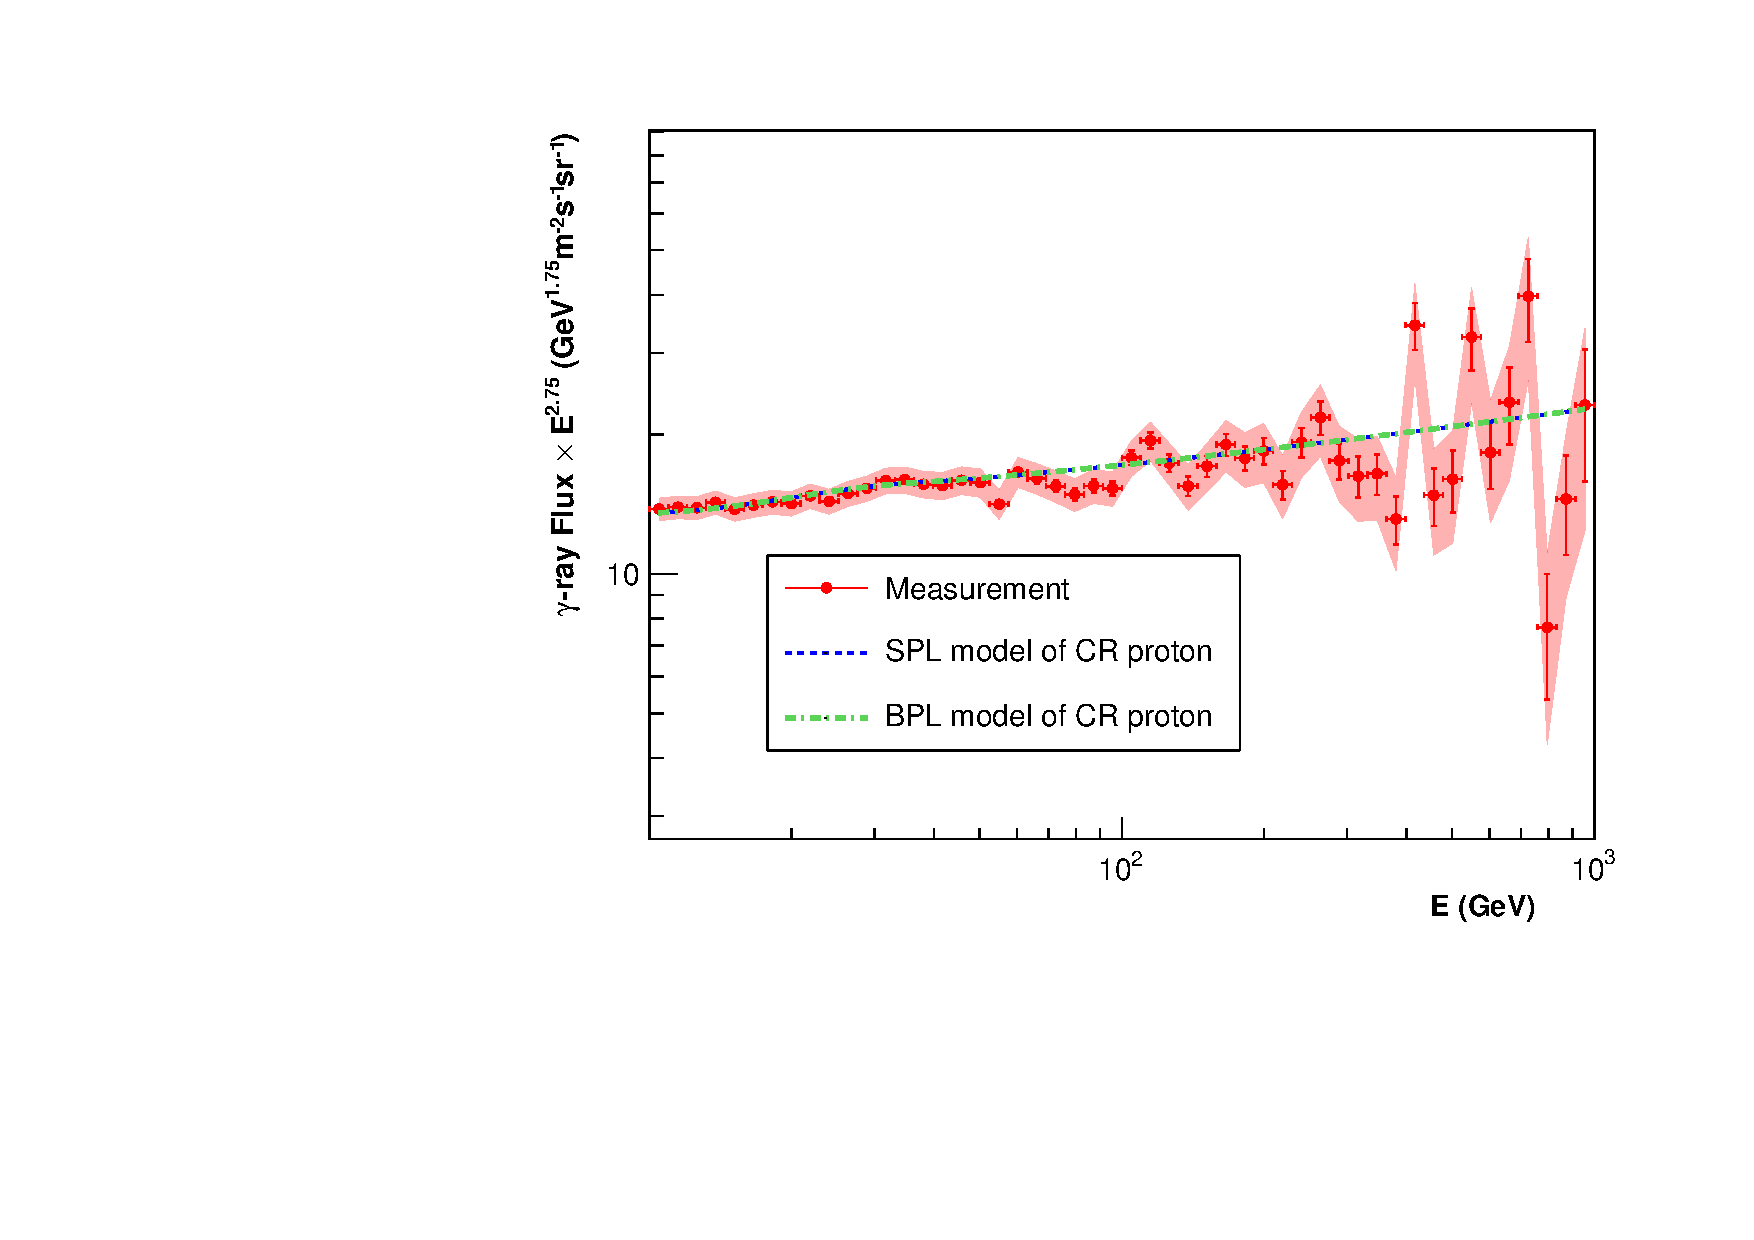
\includegraphics[width=0.8\textwidth]{content/result_and_discussion/figures/fitted_result.pdf}
    \caption{
        The Earth's $\gamma$-ray spectra calculated from the SPL (blue)
        and BPL (green) models of CR proton which best fit to the measured
        % Earth's $\gamma$-ray
        spectrum in the thin-target
        regime (red).
    }
    \label{fig:fitted_gamma_specgtrum}
\end{figure}


\begin{figure}[h!]
    \centering
    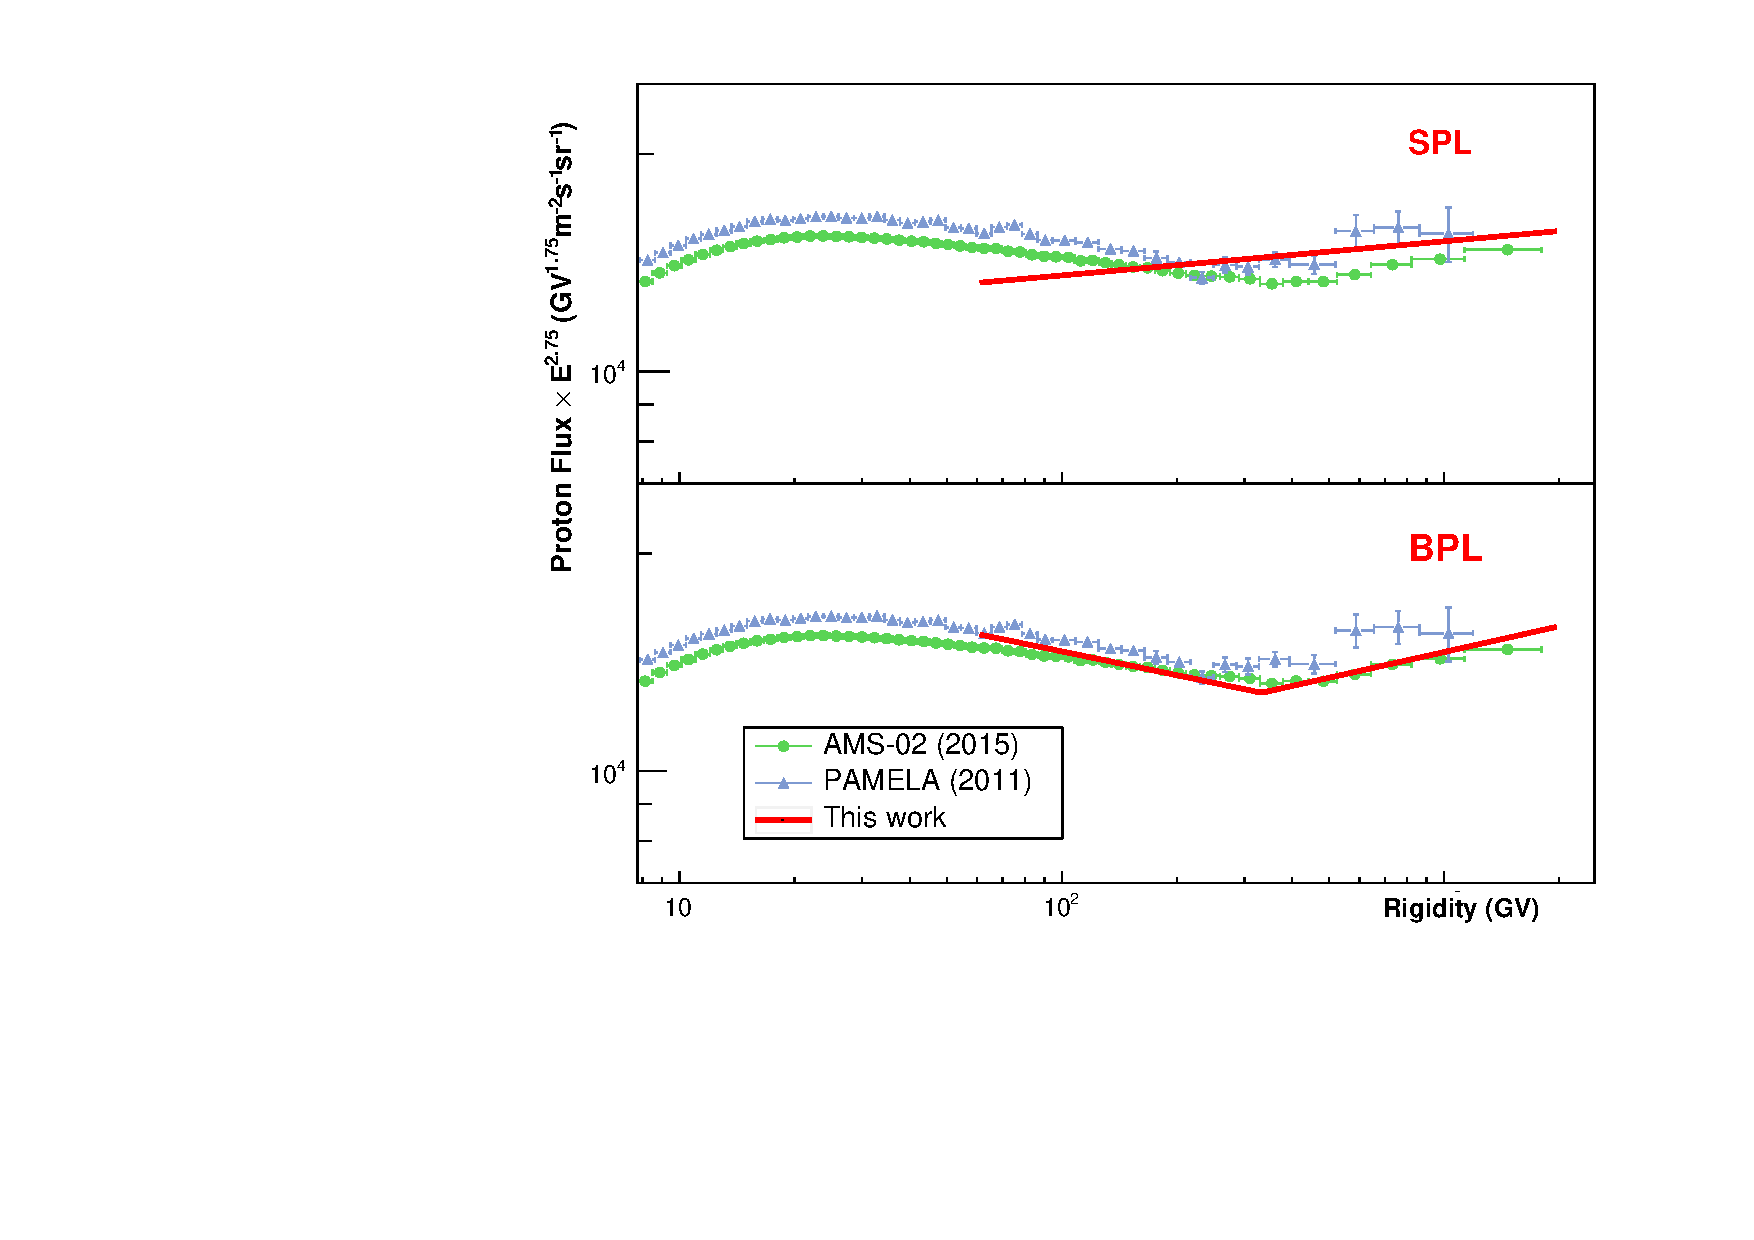
\includegraphics[width=0.9\textwidth]{content/result_and_discussion/figures/ProtonSpectrumModelMeasurement.pdf}
    \caption{
        Best-fit CR proton spectra from this work (red)
        compared to the direct measurements by AMS-02 (blue) and
        PAMELA (green).
    }
    \label{fig:fitted_cr_proton}
\end{figure}

